% Options for packages loaded elsewhere
\PassOptionsToPackage{unicode}{hyperref}
\PassOptionsToPackage{hyphens}{url}
%
\documentclass[
]{article}
\usepackage{lmodern}
\usepackage{amsmath}
\usepackage{ifxetex,ifluatex}
\ifnum 0\ifxetex 1\fi\ifluatex 1\fi=0 % if pdftex
  \usepackage[T1]{fontenc}
  \usepackage[utf8]{inputenc}
  \usepackage{textcomp} % provide euro and other symbols
  \usepackage{amssymb}
\else % if luatex or xetex
  \usepackage{unicode-math}
  \defaultfontfeatures{Scale=MatchLowercase}
  \defaultfontfeatures[\rmfamily]{Ligatures=TeX,Scale=1}
\fi
% Use upquote if available, for straight quotes in verbatim environments
\IfFileExists{upquote.sty}{\usepackage{upquote}}{}
\IfFileExists{microtype.sty}{% use microtype if available
  \usepackage[]{microtype}
  \UseMicrotypeSet[protrusion]{basicmath} % disable protrusion for tt fonts
}{}
\makeatletter
\@ifundefined{KOMAClassName}{% if non-KOMA class
  \IfFileExists{parskip.sty}{%
    \usepackage{parskip}
  }{% else
    \setlength{\parindent}{0pt}
    \setlength{\parskip}{6pt plus 2pt minus 1pt}}
}{% if KOMA class
  \KOMAoptions{parskip=half}}
\makeatother
\usepackage{xcolor}
\IfFileExists{xurl.sty}{\usepackage{xurl}}{} % add URL line breaks if available
\IfFileExists{bookmark.sty}{\usepackage{bookmark}}{\usepackage{hyperref}}
\hypersetup{
  pdftitle={Checkmate 067 study Bayesian mixture cure model analysis},
  pdfauthor={Nathan Green, Gianluca Baio, UCL},
  hidelinks,
  pdfcreator={LaTeX via pandoc}}
\urlstyle{same} % disable monospaced font for URLs
\usepackage[margin=1in]{geometry}
\usepackage{longtable,booktabs}
% Correct order of tables after \paragraph or \subparagraph
\usepackage{etoolbox}
\makeatletter
\patchcmd\longtable{\par}{\if@noskipsec\mbox{}\fi\par}{}{}
\makeatother
% Allow footnotes in longtable head/foot
\IfFileExists{footnotehyper.sty}{\usepackage{footnotehyper}}{\usepackage{footnote}}
\makesavenoteenv{longtable}
\usepackage{graphicx}
\makeatletter
\def\maxwidth{\ifdim\Gin@nat@width>\linewidth\linewidth\else\Gin@nat@width\fi}
\def\maxheight{\ifdim\Gin@nat@height>\textheight\textheight\else\Gin@nat@height\fi}
\makeatother
% Scale images if necessary, so that they will not overflow the page
% margins by default, and it is still possible to overwrite the defaults
% using explicit options in \includegraphics[width, height, ...]{}
\setkeys{Gin}{width=\maxwidth,height=\maxheight,keepaspectratio}
% Set default figure placement to htbp
\makeatletter
\def\fps@figure{htbp}
\makeatother
\setlength{\emergencystretch}{3em} % prevent overfull lines
\providecommand{\tightlist}{%
  \setlength{\itemsep}{0pt}\setlength{\parskip}{0pt}}
\setcounter{secnumdepth}{-\maxdimen} % remove section numbering
\ifluatex
  \usepackage{selnolig}  % disable illegal ligatures
\fi
\newlength{\cslhangindent}
\setlength{\cslhangindent}{1.5em}
\newlength{\csllabelwidth}
\setlength{\csllabelwidth}{3em}
\newenvironment{CSLReferences}[3] % #1 hanging-ident, #2 entry spacing
 {% don't indent paragraphs
  \setlength{\parindent}{0pt}
  % turn on hanging indent if param 1 is 1
  \ifodd #1 \everypar{\setlength{\hangindent}{\cslhangindent}}\ignorespaces\fi
  % set entry spacing
  \ifnum #2 > 0
  \setlength{\parskip}{#2\baselineskip}
  \fi
 }%
 {}
\usepackage{calc} % for \widthof, \maxof
\newcommand{\CSLBlock}[1]{#1\hfill\break}
\newcommand{\CSLLeftMargin}[1]{\parbox[t]{\maxof{\widthof{#1}}{\csllabelwidth}}{#1}}
\newcommand{\CSLRightInline}[1]{\parbox[t]{\linewidth}{#1}}
\newcommand{\CSLIndent}[1]{\hspace{\cslhangindent}#1}

\title{Checkmate 067 study Bayesian mixture cure model analysis}
\author{Nathan Green, Gianluca Baio, UCL}
\date{7 January 2021}

\begin{document}
\maketitle

\hypertarget{executive-summary}{%
\subsubsection{Executive summary}\label{executive-summary}}

In this project we formulate and demonstrate the application of a
Bayesian mixture cure model (MCM) using the Checkmate 067 study dataset
and the Exponential distribution for event times. Analogous results to
those created previously for the frequentist MCM approach are produced
and we extend the Bayesian MCM to incorporate additional structure,
including the joint (bivariate) modelling of overall survival (OS) and
progression-free survival (PFS) event times. We show that the separate
Exponential OS and PFS Bayesian MCMs perform well for the Checkmate 067
data. The jointly distributed event time Bayesian MCM also has good
predictive performance. The real benefit of this approach may be with
other dataset where there is short follow-up or small sample sizes. The
associated R code for this work, held in a private on-line repository,
has been written for re-use and generalisability to other problems.
Areas for future work are given.

\hypertarget{background}{%
\subsection{Background}\label{background}}

Immuno-oncologic (IO) studies for melanoma therapies, such as
\emph{ipilimumab} (\texttt{ipi}), \emph{nivolumab} (\texttt{nivo}), and
the \emph{nivolumab} with \emph{ipilimumab} (\texttt{nivo\ +\ ipi})
combination, have indicated that survival curves ``plateau'' (a
considerable proportion of patients are ``long-term survivors''). Cure
models are a special type of survival analysis where this ``cure
fraction'' (the underlying proportion of responders to
treatment/long-term survivors) is accounted for. Cure models estimate
the cure fraction, in addition to a parametric survival function for
patients that are not cured. The mortality risk in the cured patients is
informed by a background mortality rate. The population that is not
cured is subject both to background mortality and to additional
mortality from their cancer, estimated using a parametric survival
model.

A mixture cure model (MCM) (Amico and Van Keilegom (2018)) is a type of
cure model where survival is modelled as a mixture of two groups of
patients: those who are cured and those who are not (and who therefore
remain at risk). The survival for a population with a cure fraction can
be written as follows:

\begin{align}
\tag{*}
S(t, x) = S^*(t, x)[\pi(x) + (1 − \pi(x))S_u(t, x)],
\end{align}

where \(S(t, x)\) denotes the survival at time \(t\), \(S^*(t, x)\)
denotes the background mortality at time \(t\) conditional on covariates
\(x\), \(\pi(x)\) denotes the probability of being cured conditional on
covariates \(x\), and \(S_u(t, x)\) denotes the event (progression or
mortality) due to cancer at time \(t\) conditional on covariates \(x\).
For PFS, the survival is composed of either progressing to a disease
state or death.

\hypertarget{aims}{%
\subsection{Aims}\label{aims}}

The aims of the the analysis in this document are as follows:

\begin{itemize}
\tightlist
\item
  Demonstrate the application of a Bayesian mixture cure model using the
  Checkmate 067 study dataset and the Exponential distribution for event
  times.
\item
  Produce analogous results to those created previously for the
  frequentist approach.
\item
  Extend the Bayesian model to incorporate additional structure,
  including the joint bivariate modelling of OS and PFS event times.
\end{itemize}

This analysis has been carried-out using the Stan inference engine
(Carpenter et al. (2017)) called from R on a Windows PC. The packaged
code can be downloaded from a private GitHub repository with permission
from the package authors at
\url{https://github.com/StatisticsHealthEconomics/rstanbmcm}. See the
\emph{How to use rstanbmcm} vignette for an introduction to how to use
the package.

\hypertarget{likelihood}{%
\subsection{Likelihood}\label{likelihood}}

Let \(T_i\) be the non-negative random variable denoting the survival
time of patient \(i\) with covariate vector \(\boldsymbol{x}_i\).

In the simplest case we can assume that the cure fraction is the same
for the whole population i.e.~\(\pi\) is fixed. Further, we can assume
the \(\pi\) models the relationship between \(\boldsymbol{x}_i\) and the
probability of being cured. E.g. using a logistic-linear model

\[
\pi(\boldsymbol{x}_i | \boldsymbol{\beta}) = 1/[1 + \exp(-\boldsymbol{x}_i^T \boldsymbol{\beta})].
\]

The likelihood of the standard survival is

\[
L = \prod_i S(t_i | \boldsymbol{x}_i) h(t_i | \boldsymbol{x}_i)^{\delta_i}
\]

Log-likelihood is therefore \[
\mathcal{l} = \sum_i \log(S(t_i | \boldsymbol{x}_i)) + \delta_i \log(h(t_i | \boldsymbol{x}_i))
\]

Plugging this directly into the mixture cure equation in (*) gives

\[
\mathcal{l}(\pi | \boldsymbol{\delta}, \boldsymbol{x}) =
 \sum_i \log(S^*(t_i | \boldsymbol{x}_i) h^*(t_i | \boldsymbol{x}_i)^{\delta_i}[\pi(x) +
   (1 − \pi(x)) S_u(t_i | \boldsymbol{x}_i) h_u(t_i | \boldsymbol{x}_i)^{\delta_i}])
\]

We will assume that the cured component is the exponential survival
model. The non-cured component can be thought of in similar terms to the
cumulative incidence function. That is, the probability of an event is
the combined probability of surviving both events (e.g.~for OS,
all-cause and cancer mortality) and then experiencing either i.e.
dropping the \(S\) dependencies for brevity

\begin{equation}
\tag{**}
S^* S_u (h^*)^{\delta} + S^* S_u (h_u)^{\delta} = S^* S_u (h^* + h_u)^{\delta}
\end{equation}

\hypertarget{bayesian-formulation}{%
\subsection{Bayesian formulation}\label{bayesian-formulation}}

In a Bayesian approach to modelling, all quantities that are subject to
uncertainty are modelled using probability distributions. This applies
to observed data (e.g.~time to PFS for a given individual), that are
subject to sampling variability, as well as to unobservable parameters
(e.g.~the coefficient quantifying the impact of age or sex over the
average survival curve). In this latter case, probability distributions
are used to model the epistemic uncertainty (e.g.~the fact that we do
not know for certain what the ``true'' underlying value of the model
parameter is). In addition, we may model as yet unobserved (but
potentially observable) quantities using a suitable probability model.
For example, we could consider the extrapolated part of the survival
curve as subject to uncertainty due to the current sampling process
giving rise to the data that are actually observed, as well as the
uncertainty on the underlying data generating process.

We can mix different sources of evidence to form our ``prior''
distributions, which are used to describe the state of science on the
model parameters. These are then combined with any observed data to form
an updated level of knowledge. This process is particularly relevant in
the case at hand, when data can only inform about limited aspects of the
overall underlying reality. For this reason, it is important to a)
include information/evidence available in the form of external data
and/or expert opinion; b) extract the most information possible from the
available data (e.g.~by formally trying to model the correlation between
the PFS and the OS data to borrow strength from the more mature set of
observations).

A built-in advantage of the Bayesian procedure is that uncertainty is
directly and formally propagated to an economic model; the main output
from the statistical analysis (the extrapolated survival curve) are
produced by default as based on a full posterior distribution. From
this, we can easily derive a ``base case'' (e.g.~taking the mean value)
but without the need for further tools (such as bootstrap) we already
have a full characterisation of the underlying uncertainty that can be
used in the process of probabilistic sensitivity analysis. We can
moreover add information in the priors to ensure that the extrapolation
beyond the observed data is realistic and consistent with the clinical
expertise (e.g.~by ``anchoring'' the extrapolated survival curve to be
probabilistically below the curves for the healthy population, or by
ensuring that OS behaves in a way to respect some agreed level of
similarity, or correlation, to PFS).

\hypertarget{posterior-equation}{%
\paragraph{Posterior equation}\label{posterior-equation}}

Using the likelihood function defined above and prior distributions on
uncertain parameters, we can specify the posterior distribution.
Defining \(g_2\) as the prior distribution for the coefficients of the
uncured fraction \(\beta^u\) and \(g_3\) as the prior distribution for
the coefficients of the cured fraction \(\beta^*\), then the general
form of the posterior distribution can be written as follows.

\[
p(\pi, \boldsymbol{\beta^u}, \boldsymbol{\beta^*} | \boldsymbol{\delta}, \boldsymbol{x}) \propto
L(\pi, \boldsymbol{\beta^u}, \boldsymbol{\beta^*} | \boldsymbol{\delta}, \boldsymbol{x}) f(\pi) g_2(\boldsymbol{\beta^u}) g_3(\boldsymbol{\beta^*})
\]

assuming that the cure fraction is independent of the covariates.

\hypertarget{cure-fraction}{%
\subsubsection{Cure fraction}\label{cure-fraction}}

There are two obvious ways to represent the uncertainty about the cure
fraction in the model.

The first is to specify the cure fraction directly using a
\(\pi \sim Beta(a_{cf}, b_{cf})\) prior, most uninformative as a uniform
\(Beta(1,1)\). The parameters can be obtained via transformation of mean
and standard deviation to allow a more natural scale for elicitation.

Alternatively, we may specify the uncertainty on the real line with a
Normal distribution and then transform to the probability scale.

A further consideration is how to represent the cure fraction so to
share information between the OS and PFS data. We will investigate 3
alternatives.

\begin{itemize}
\tightlist
\item
  \emph{Pooled}: Assume that the cure fraction is the same for OS and
  PFS i.e.~\(\pi_{os} = \pi_{os} = \pi\) where \[
  logit(\pi) \sim N(\mu_{cf}, \sigma_{cf}^2), \;\;
  \]
\item
  \emph{Separate}: Model each independently. \[
  logit(\pi_{os}) \sim N(\mu_{cfos}, \sigma_{cfos}^2), \;\;  
  logit(\pi_{pfs}) \sim N(\mu_{cfpfs}, \sigma_{cfpfs}^2)  
  \]
\item
  \emph{Hierarchical}: Assume exchangeability between OS and PFS\[
  \pi \sim N(\mu_{cf}, \sigma_{cf}^2), \;\;  
  logit(\pi_{os}) \sim N(\pi, \sigma_{cfos}^2), \;\;  
  logit(\pi_{pfs}) \sim N(\pi, \sigma_{cfpfs}^2)  
  \]
\end{itemize}

Below is an example DAG for the hierarchical cure fraction without a
joint time to event component. Notice that even without the direct
relationship between PFS and OS there is still an indirect influence via
\(\pi\).

\begin{center}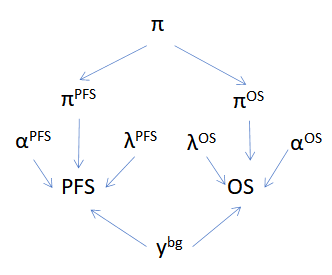
\includegraphics[width=0.4\linewidth]{hierarchical_DAG} \end{center}

\hypertarget{exponentially-distributed-event-times}{%
\subsection{Exponentially distributed event
times}\label{exponentially-distributed-event-times}}

Consider the straightforward case where both the background and cancer
times to event follow Exponential distributions.

Define \(f(t)\) density, \(S(t)\) survival and \(h(t)\) hazard
functions.

\[
f(t) = \lambda \exp(-\lambda t), \;\; S(t) = \exp(-\lambda t), \;\; h(t) = \lambda
\]

Which gives the likelihood

\[
\mathcal{l}(\pi | \boldsymbol{\delta}, \boldsymbol{x}) =
 \sum_i \log(\exp(-\lambda^* t) \lambda^{* \delta_i}[\pi(x) +
   (1 − \pi(x)) \exp(-\lambda_u t) \lambda_u^{\delta_i}])
\]

Substituting \(S(t)\) and \(h(t)\) into (**)

\[
f^*_u = e^{-\lambda^* t} e^{-\lambda_u t} (\lambda^* + \lambda_u)^{\delta} \;\;\; i.e. \mbox{for no censoring} \;\; T \sim Exp(\lambda^* + \lambda_u)
\]

\hypertarget{background-survival}{%
\subsection{Background survival}\label{background-survival}}

The frequentist analysis used the World Health Organization (WHO) life
tables by country for the latest year available of 2016 (WHO (2020)) to
inform the background mortality rate (baseline hazard). These baseline
hazards are the expected mortality rate for each patient at the age at
which they experience the event. The mortality data are age- and gender
adjusted, thus providing a granular account of the different patient
profiles in the trial. The WHO reports conditional probabilities of
death in 5-year intervals until age 85. A constant annual mortality rate
is reported for individuals over 85. They assumed that the maximum age
is 100 years.

In a Bayesian analysis there are alternative ways in which we could
model the background mortality.

\hypertarget{use-who-hazard-point-estimates-as-known}{%
\paragraph{Use WHO hazard point estimates as
known}\label{use-who-hazard-point-estimates-as-known}}

We could consider the WHO estimates to provide sufficiently accurate
estimates given the sample size and so incorporating uncertainty is not
necessary.

\hypertarget{survival-distribution-informed-by-the-who-data}{%
\paragraph{Survival distribution informed by the WHO
data}\label{survival-distribution-informed-by-the-who-data}}

However, we also want the developed model to be able to be applied to
other data sets which may be smaller or noisy. Also the mortality rate
for the cured study population may not be the same as the general
population. Sensible prior parameter values can be taken for the life
table hazard curve. After infancy the log-hazard is approximately linear
and so intercept and slope estimates are simple to obtain.

In this analysis we use the more general distributional approach. This
allows for more freedom in the model fitting.

\hypertarget{jointly-distributed-event-times-model}{%
\subsection{Jointly distributed event times
model}\label{jointly-distributed-event-times-model}}

One effective way of modelling joint (bivariate) distributions is to
factorise them into a marginal and a conditional distribution (which
holds as a fundamental rule of probability). In general terms, we can
then write \(p(x,y) = p(x)p(y | x)\). In the context of our model, we
can use this intuition to model the joint distribution of the PFS and OS
observed times (in terms of their survival curves) as: \[
S(t_{OS},t_{PFS}) = P⁡(T_{OS} \geq t_{OS}, T_{PFS} \geq t_{PFS})
= S_{PFS} (t_{PFS}) S_{OS|PFS}(t_{OS}│T_{PFS} = t_{PFS}).
\] The structure above implies that essentially we first create a
marginal generalised linear regression to model the survival curve for
the PFS data (as a function of relevant covariates); the second module
of the model implies another generalised linear regression for the OS
data, where the observed PFS data act as a covariate (in addition to
other relevant predictors, which may or may not be the same used for the
PFS model). Alternative specifications are possible (for instance, the
generalised linear model can be applied on the scale of the hazard
function, if more appropriate). This modelling approach can be
visualised in the graph below.

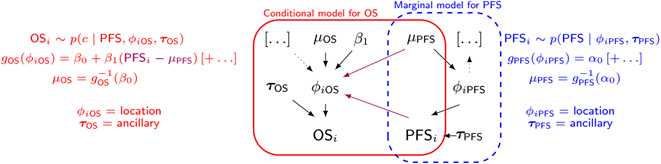
\includegraphics[width=0.8\textwidth,height=\textheight]{DAG.png}

If we factorise into marginal and conditional components to model the
underlying bivariate distribution this can be written generally as

\[
OS_i \sim p(c | PFS, \phi_{iOS}, \tau_{OS})
\] \[
g_{OS}(\phi_{iOS}) = \beta_0 + \beta_1 (PFS_i - \mu_{PFS})[+ \ldots]
\] \[
\mu_{OS} = g_{OS}^{-1}(\beta_0)
\] \[
g_{PFS}(\phi_{iPFS}) = \alpha_0 [+ \ldots]
\] \[
PFS_i \sim p(PFS | \phi_{iPFS}, \tau_{PFS})
\] \[
\mu_{PFS} = g_{PFS}^{-1}(\alpha_0)
\]

The combined log-likelihood is \[
\mathcal{l} = \mathcal{l}_{OS} + \mathcal{l}_{PFS}
\]

For the case with exponential OS times and exponential PFS times with
centred age this gives the following.

\[
t_{iOS} \sim Exp(\phi_{iOS})
\] \[
\log(\phi_{iOS}) = \beta_0 + \beta_1 (t_{iPFS} - \bar{t}_{PFS}) + \beta_2 age_{iPFS}
\] \[
\mu_{OS} = \exp(\beta_0)
\] \[
\log(\phi_{iPFS}) = \alpha_0 + \alpha_1 age_{iOS}
\] \[
t_{iPFS} \sim Exp(\phi_{iPFS})
\] \[
\mu_{PFS} = \exp(\alpha_0)
\] \[
\bar{t}_{PFS} = 1/\mu_{PFS} 
\]

Where \(\bar{t}_{PFS}\) is the mean time to event for PFS. This is
simple to calculate for the Exponential distribution but is more
complicated for other survival distributions. The parameters
\(\phi_{iOS}\) and \(\phi_{iPFS}\) are the uncured hazard rates for
individual \(i\) for OS and PFS, respectively.

The background hazard rates are specified as follows

\[
t_{iOS} \sim Exp(\phi^*_{iOS})
\] \[
\log(\phi^*_{iOS}) = \beta_0^* + \beta^*_1 age_{iOS}
\] \[
t_{iPFS} \sim Exp(\phi^*_{iPFS})
\] \[
\log(\phi^*_{iPFS}) = \beta_0^* + \beta^*_1 age_{iPFS}
\] Notice that the coefficients \(\beta_0^*\) and \(\beta^*_1\) are the
same in both equations .

\hypertarget{results}{%
\subsection{Results}\label{results}}

We fit the exponential hazard model to the study data and produced the
posterior survival curves below.

For each model and treatment we produce two figures:

\begin{enumerate}
\def\labelenumi{\arabic{enumi}.}
\item
  The expected survival curves with 95\% Credible Intervals (CrI). The
  OS curves are to the left-hand side and PFS curves to the right-hand
  side. Background mortality (i.e.~cured patients) is indicated by the
  red line. Non-cured patients survival curves are shown in dark green
  and blue for OS and PFS respectively. Light green and magenta are the
  total sample. The black line is the Kaplan-Meier curve for the
  observed data. Note that these plots are for an average individual,
  e.g.~at average age, and so we would not expect them to perfectly
  match the sample data Kaplan-Meier.
\item
  Kaplan-Meier curves for 50 simulated trials using the posterior
  prediction distribution for time to event. This is a good model
  checking plot, indicating if we can replicate data similar to the
  observed data using the fitted model.
\end{enumerate}

For the Checkmate dataset we found that the hierarchical model gave
equivalent results to the separate cure fraction model and so for speed
of computation and simplicity we only show the separate cure fraction
results here.

\hypertarget{independent-pfs-and-os-event-times-distributional-background}{%
\subsubsection{Independent PFS and OS event times, distributional
background}\label{independent-pfs-and-os-event-times-distributional-background}}

\hypertarget{pooled-cure-fraction}{%
\paragraph{Pooled cure fraction}\label{pooled-cure-fraction}}

This is the most restrictive model and so as we would expect it gives
the worse results. The OS appears better than the PFS plots; the PFS
CrIs fail to contain the observed data.

\begin{center}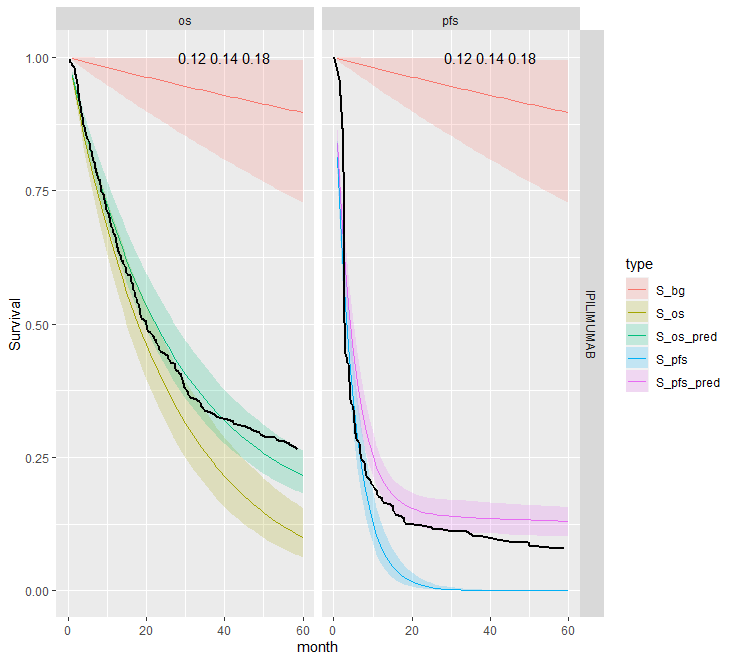
\includegraphics[width=0.4\linewidth]{../plots/S_plots_exp_exp_cf_pooled_IPI} 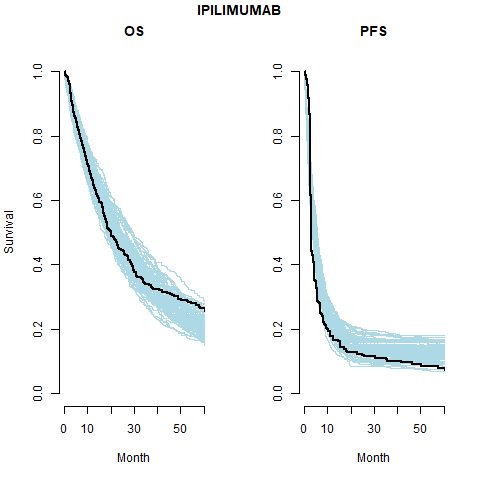
\includegraphics[width=0.4\linewidth]{../plots/post_pred_cf pooled_exp_exp_IPILIMUMAB} \end{center}

\begin{center}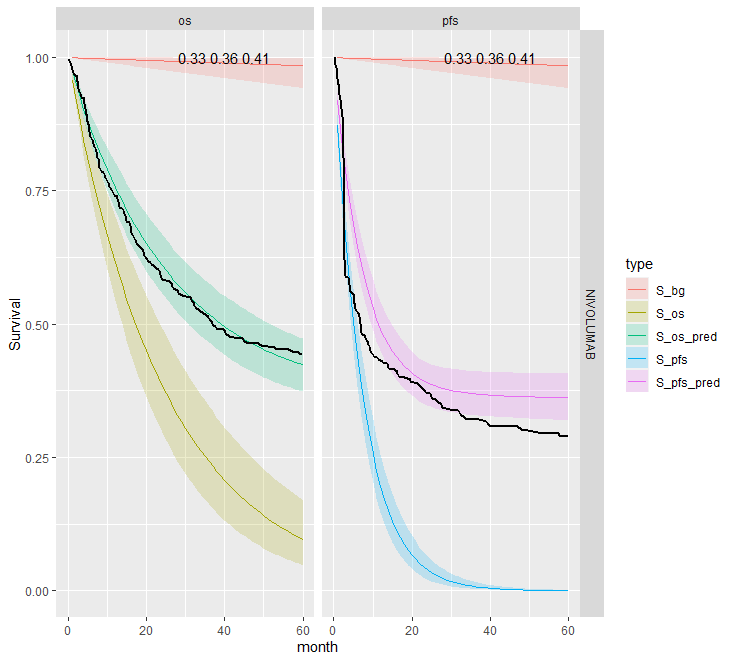
\includegraphics[width=0.4\linewidth]{../plots/S_plots_exp_exp_cf_pooled_NIVO} 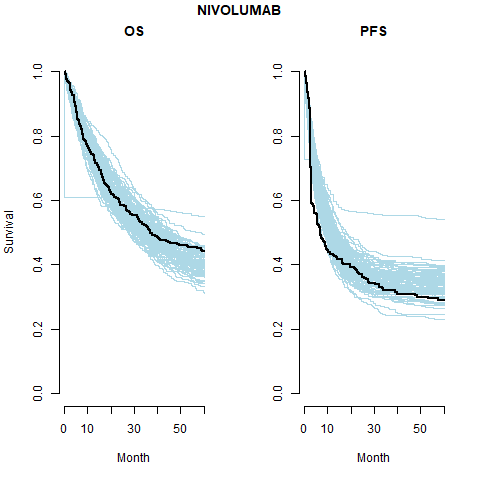
\includegraphics[width=0.4\linewidth]{../plots/post_pred_cf pooled_exp_exp_NIVOLUMAB} \end{center}

\begin{center}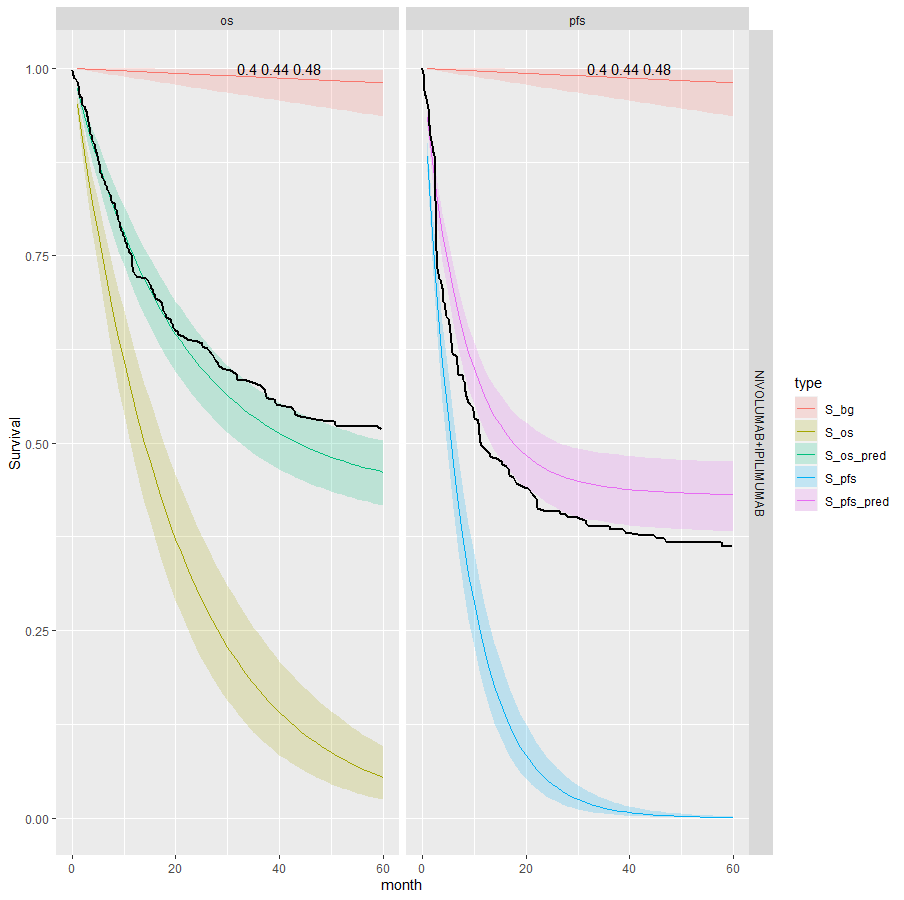
\includegraphics[width=0.4\linewidth]{../plots/S_plots_exp_exp_cf_pooled_NIVO+IPI} 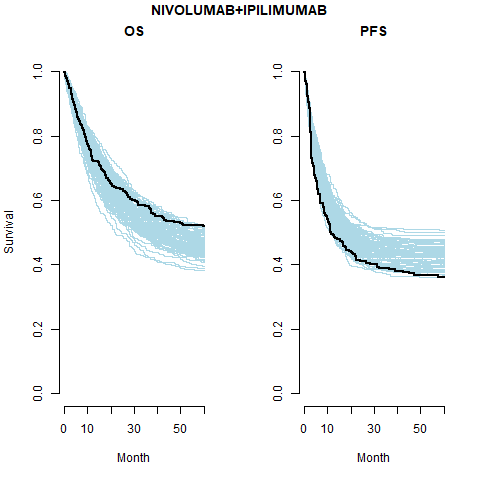
\includegraphics[width=0.4\linewidth]{../plots/post_pred_cf pooled_exp_exp_NIVOLUMAB+IPILIMUMAB} \end{center}

\hypertarget{separate-cure-fraction}{%
\paragraph{Separate cure fraction}\label{separate-cure-fraction}}

The models with independently fit cure fraction appear to fit reasonably
well. The mismatch in fit is due to the assumption of an exponential
survival curve for uncured patients which does not capture the true
curvature.

\begin{center}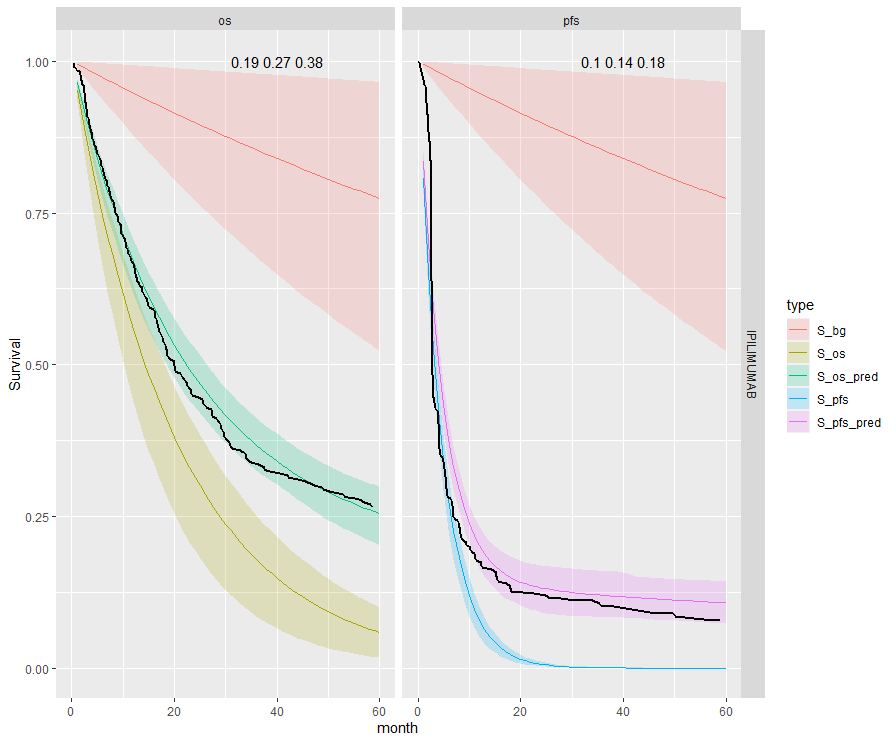
\includegraphics[width=0.4\linewidth]{../plots/S_plots_exp_exp_cf_separate_IPI} 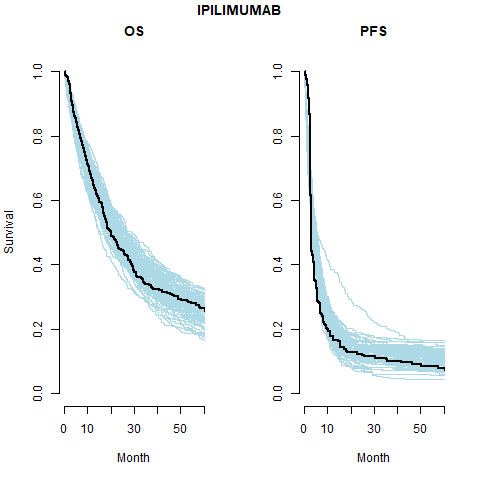
\includegraphics[width=0.4\linewidth]{../plots/post_pred_cfsep_exp_exp_IPILIMUMAB} \end{center}

\begin{center}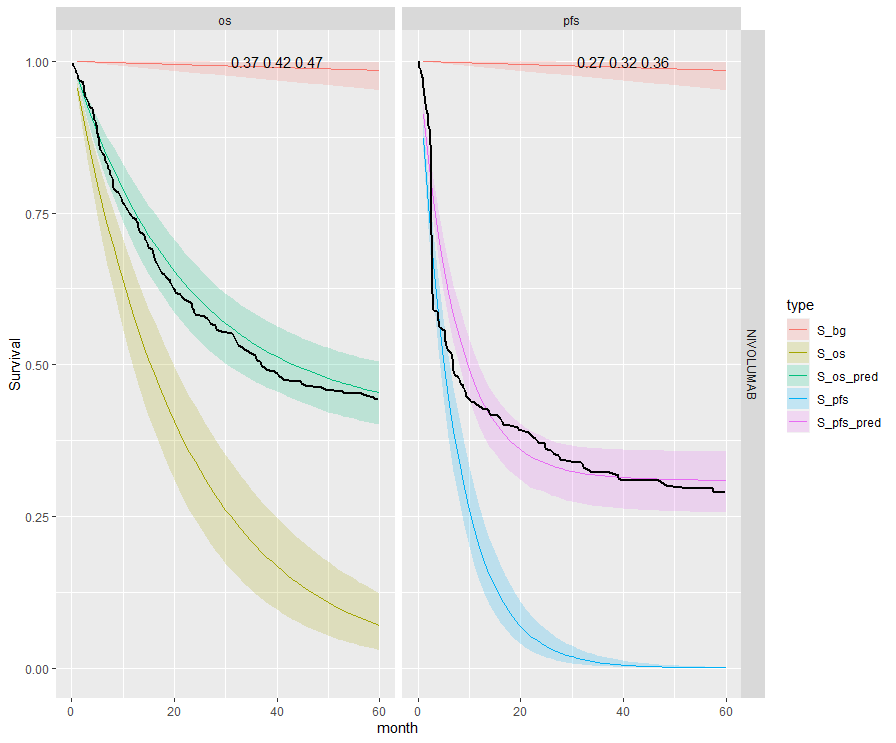
\includegraphics[width=0.4\linewidth]{../plots/S_plots_exp_exp_cf_separate_NIVO} 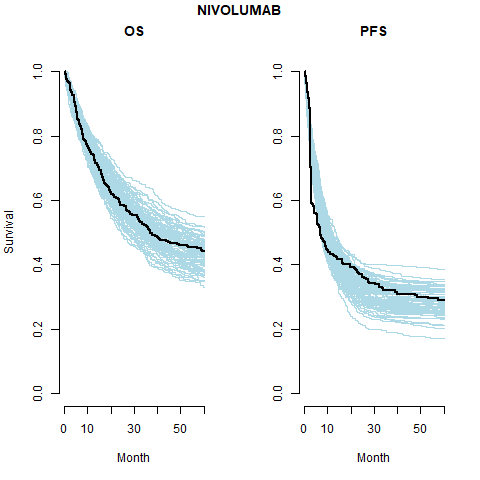
\includegraphics[width=0.4\linewidth]{../plots/post_pred_cfsep_exp_exp_NIVOLUMAB} \end{center}

\begin{center}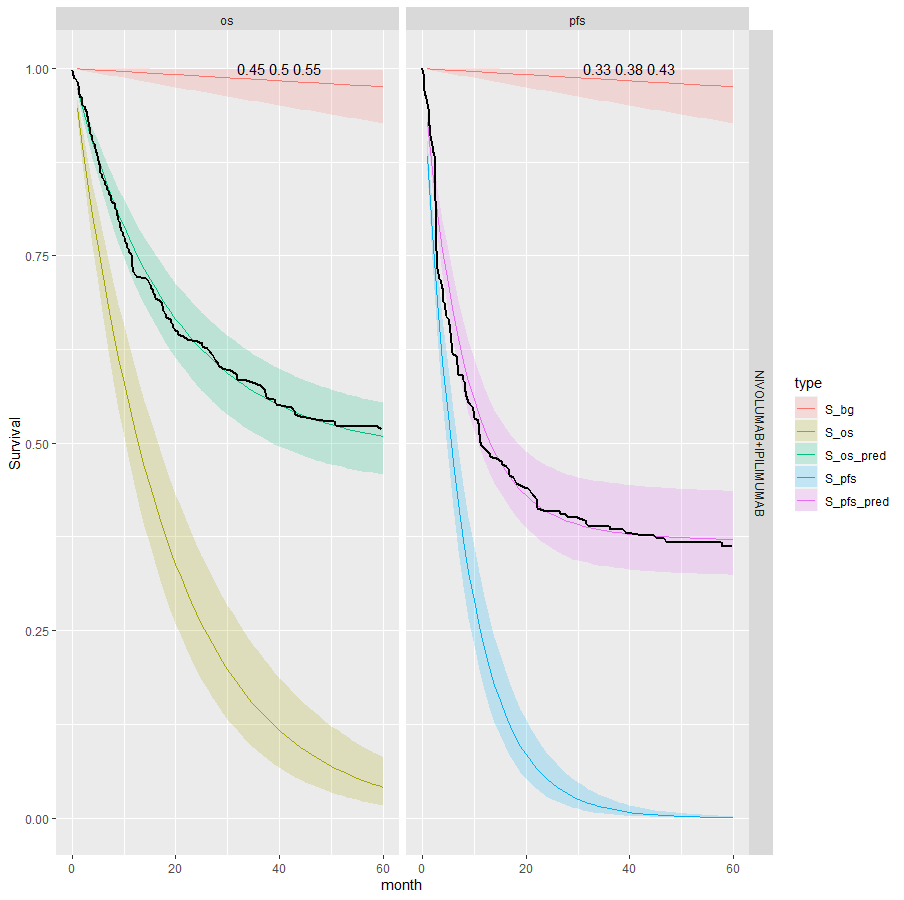
\includegraphics[width=0.4\linewidth]{../plots/S_plots_exp_exp_cf_separate_NIVO+IPI} 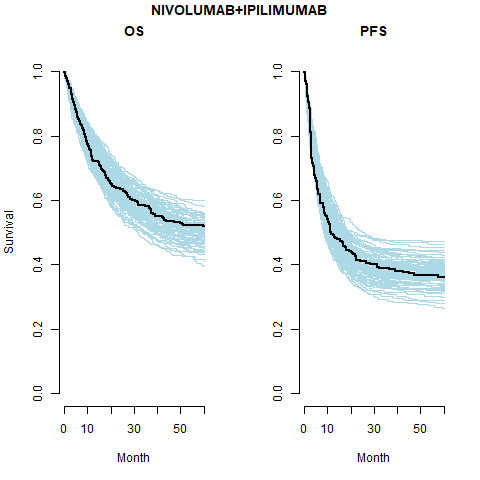
\includegraphics[width=0.4\linewidth]{../plots/post_pred_cfsep_exp_exp_NIVOLUMAB+IPILIMUMAB} \end{center}

\hypertarget{jointly-distributed-pfs-and-os-event-times-distributional-background}{%
\subsubsection{Jointly distributed PFS and OS event times,
distributional
background}\label{jointly-distributed-pfs-and-os-event-times-distributional-background}}

We see that the expected OS survival curves are biased; over-estimating
the rate. This is not the case for the \emph{ipilimumab}. This is due to
the additional joint component in the OS linear regression. This may be
due to censoring since \emph{ipilimumab} has the smallest amount. This
is an area for research.

However, the model does fit well taking in to account the case-mix of
the study population. The posterior prediction plots show that the
Kaplan-Meier for the observed data lies within the simulated curves.

\begin{center}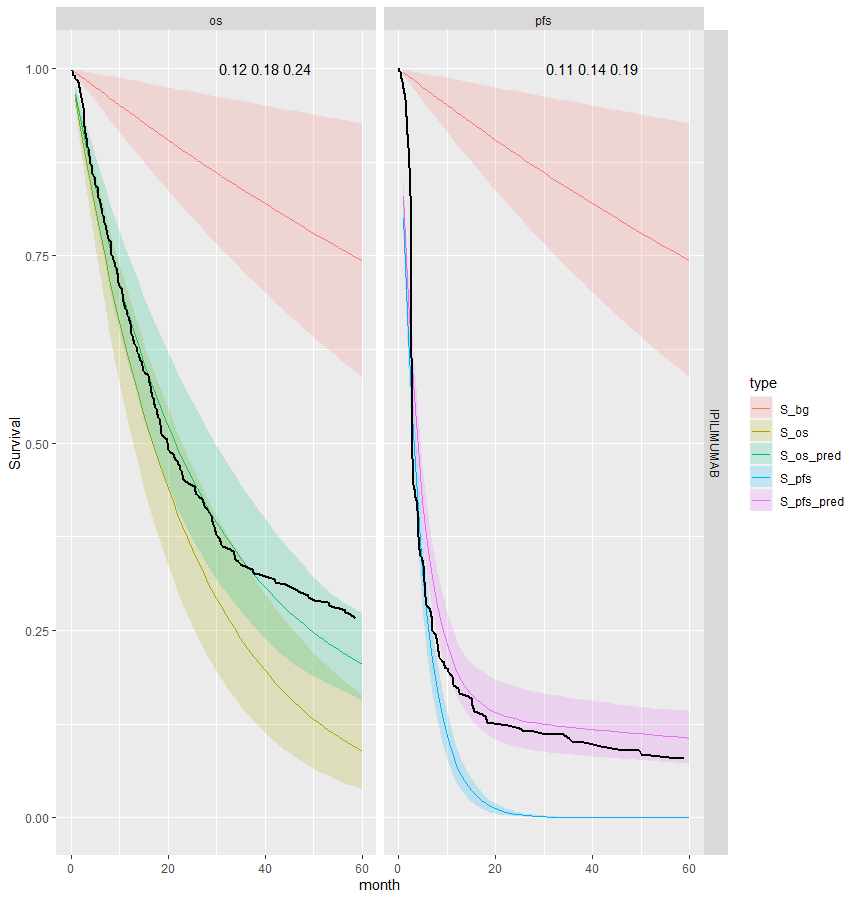
\includegraphics[width=0.4\linewidth]{../plots/S_plots_exp_exp_cf_separate_IPI_joint} 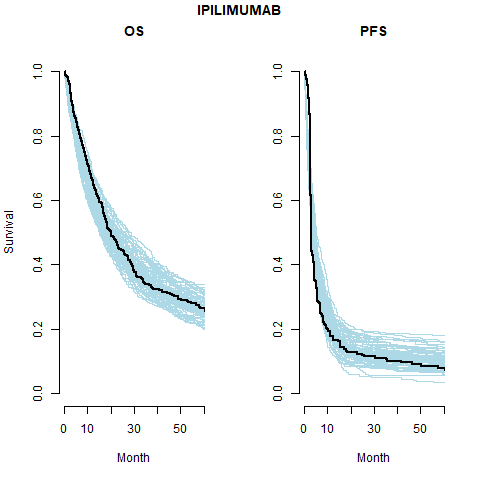
\includegraphics[width=0.4\linewidth]{../plots/post_pred_joint_cf separate_exp_exp_IPILIMUMAB} \end{center}

\begin{center}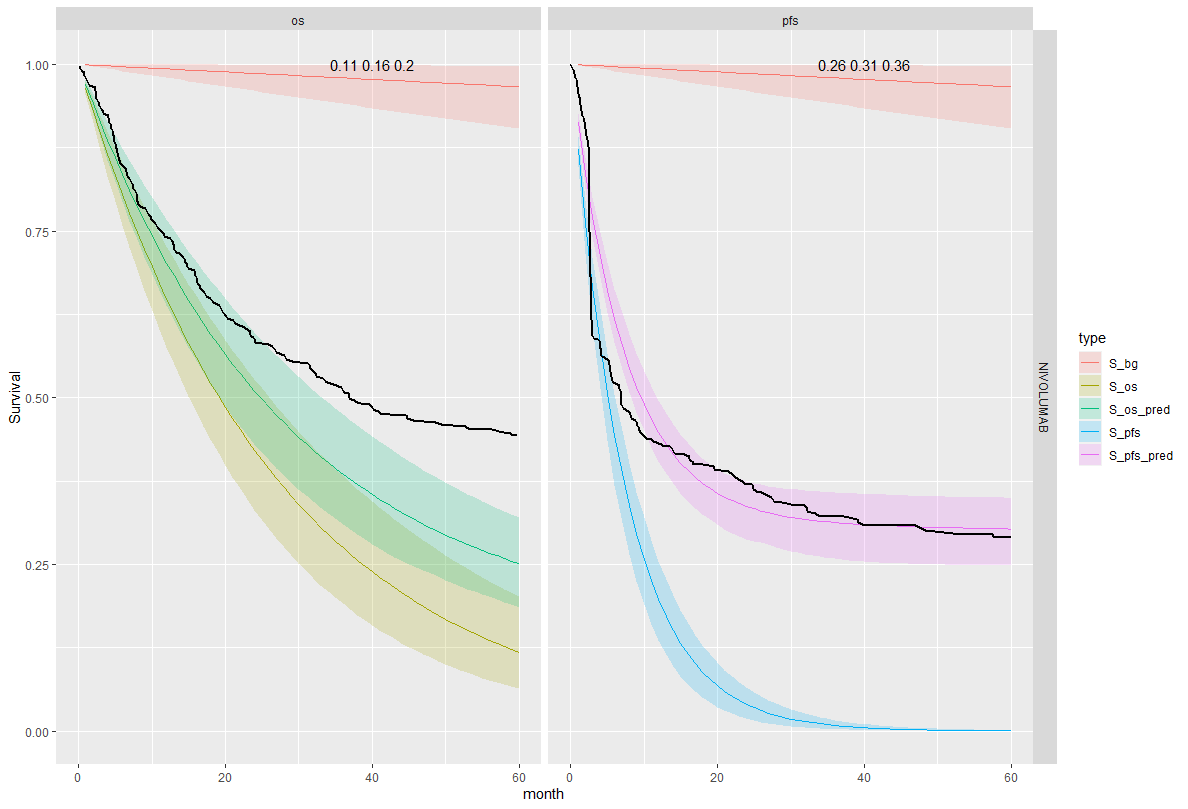
\includegraphics[width=0.4\linewidth]{../plots/S_plots_exp_exp_cf_separate_NIVO_joint} 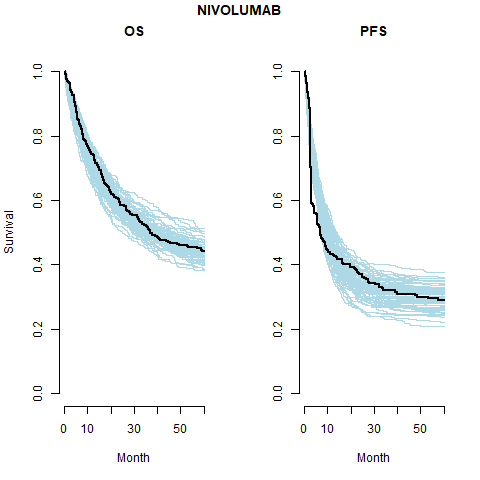
\includegraphics[width=0.4\linewidth]{../plots/post_pred_joint_cf separate_exp_exp_NIVOLUMAB} \end{center}

\begin{center}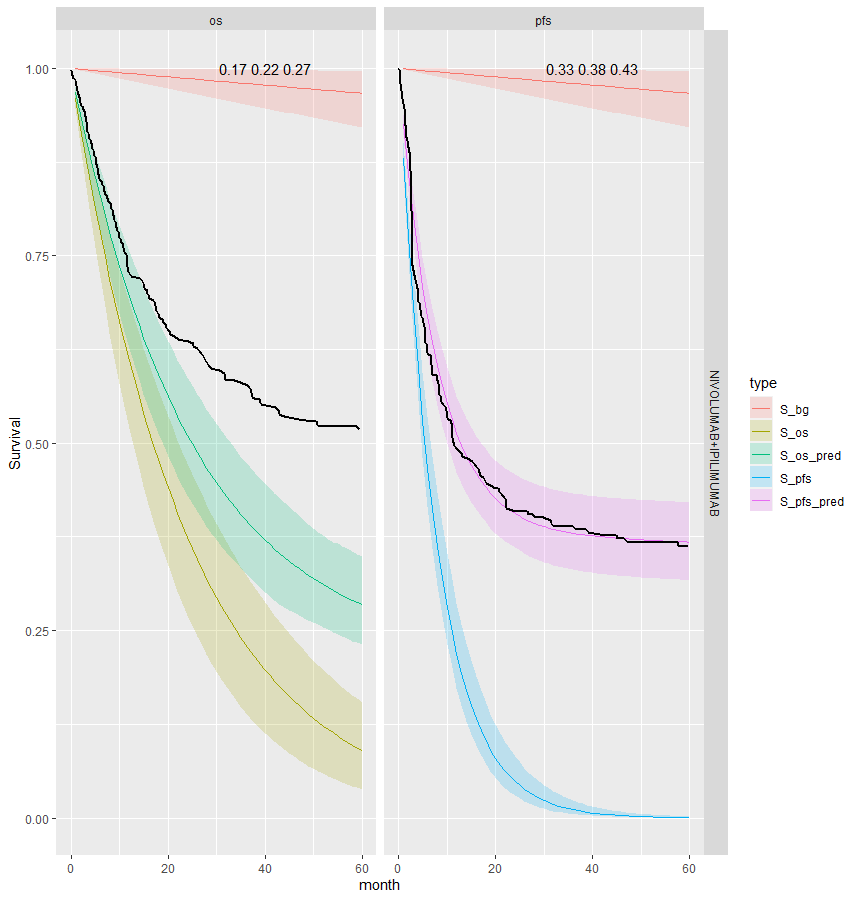
\includegraphics[width=0.4\linewidth]{../plots/S_plots_exp_exp_cf_separate_NIVO+IPI_joint} 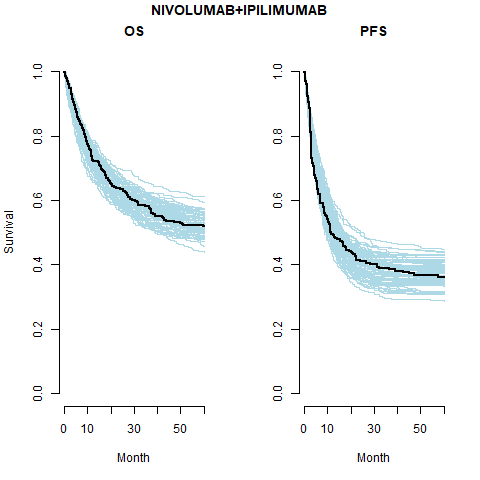
\includegraphics[width=0.4\linewidth]{../plots/post_pred_joint_cf separate_exp_exp_NIVOLUMAB+IPILIMUMAB} \end{center}

The table below summarises the cure fraction posterior distribution for
each scenario.

\begin{longtable}[]{@{}lrrrrrr@{}}
\toprule
\begin{minipage}[b]{0.01\columnwidth}\raggedright
\strut
\end{minipage} & \begin{minipage}[b]{0.10\columnwidth}\raggedleft
Event times\strut
\end{minipage} & \begin{minipage}[b]{0.12\columnwidth}\raggedleft
Cure fraction\strut
\end{minipage} & \begin{minipage}[b]{0.09\columnwidth}\raggedleft
Treatment\strut
\end{minipage} & \begin{minipage}[b]{0.15\columnwidth}\raggedleft
\(cf_{OS}\) (CrI)\strut
\end{minipage} & \begin{minipage}[b]{0.15\columnwidth}\raggedleft
\(cf_{PFS}\) (CrI)\strut
\end{minipage} & \begin{minipage}[b]{0.19\columnwidth}\raggedleft
\(\beta_{joint}\) (CrI)\strut
\end{minipage}\tabularnewline
\midrule
\endhead
\begin{minipage}[t]{0.01\columnwidth}\raggedright
1\strut
\end{minipage} & \begin{minipage}[t]{0.10\columnwidth}\raggedleft
Independent\strut
\end{minipage} & \begin{minipage}[t]{0.12\columnwidth}\raggedleft
Pooled\strut
\end{minipage} & \begin{minipage}[t]{0.09\columnwidth}\raggedleft
IPI\strut
\end{minipage} & \begin{minipage}[t]{0.15\columnwidth}\raggedleft
0.14 (0.12, 0.18)\strut
\end{minipage} & \begin{minipage}[t]{0.15\columnwidth}\raggedleft
0.14 (0.12, 0.18)\strut
\end{minipage} & \begin{minipage}[t]{0.19\columnwidth}\raggedleft
\strut
\end{minipage}\tabularnewline
\begin{minipage}[t]{0.01\columnwidth}\raggedright
2\strut
\end{minipage} & \begin{minipage}[t]{0.10\columnwidth}\raggedleft
Independent\strut
\end{minipage} & \begin{minipage}[t]{0.12\columnwidth}\raggedleft
Pooled\strut
\end{minipage} & \begin{minipage}[t]{0.09\columnwidth}\raggedleft
NIVO\strut
\end{minipage} & \begin{minipage}[t]{0.15\columnwidth}\raggedleft
0.36 (0.33, 0.41)\strut
\end{minipage} & \begin{minipage}[t]{0.15\columnwidth}\raggedleft
0.36 (0.33, 0.41)\strut
\end{minipage} & \begin{minipage}[t]{0.19\columnwidth}\raggedleft
\strut
\end{minipage}\tabularnewline
\begin{minipage}[t]{0.01\columnwidth}\raggedright
3\strut
\end{minipage} & \begin{minipage}[t]{0.10\columnwidth}\raggedleft
Independent\strut
\end{minipage} & \begin{minipage}[t]{0.12\columnwidth}\raggedleft
Pooled\strut
\end{minipage} & \begin{minipage}[t]{0.09\columnwidth}\raggedleft
NIVO+IPI\strut
\end{minipage} & \begin{minipage}[t]{0.15\columnwidth}\raggedleft
0.44 (0.4, 0.48)\strut
\end{minipage} & \begin{minipage}[t]{0.15\columnwidth}\raggedleft
0.44 (0.4, 0.48)\strut
\end{minipage} & \begin{minipage}[t]{0.19\columnwidth}\raggedleft
\strut
\end{minipage}\tabularnewline
\begin{minipage}[t]{0.01\columnwidth}\raggedright
4\strut
\end{minipage} & \begin{minipage}[t]{0.10\columnwidth}\raggedleft
Independent\strut
\end{minipage} & \begin{minipage}[t]{0.12\columnwidth}\raggedleft
Separate\strut
\end{minipage} & \begin{minipage}[t]{0.09\columnwidth}\raggedleft
IPI\strut
\end{minipage} & \begin{minipage}[t]{0.15\columnwidth}\raggedleft
0.27 (0.19, 0.38)\strut
\end{minipage} & \begin{minipage}[t]{0.15\columnwidth}\raggedleft
0.14 (0.1, 0.18)\strut
\end{minipage} & \begin{minipage}[t]{0.19\columnwidth}\raggedleft
\strut
\end{minipage}\tabularnewline
\begin{minipage}[t]{0.01\columnwidth}\raggedright
5\strut
\end{minipage} & \begin{minipage}[t]{0.10\columnwidth}\raggedleft
Independent\strut
\end{minipage} & \begin{minipage}[t]{0.12\columnwidth}\raggedleft
Separate\strut
\end{minipage} & \begin{minipage}[t]{0.09\columnwidth}\raggedleft
NIVO\strut
\end{minipage} & \begin{minipage}[t]{0.15\columnwidth}\raggedleft
0.42 (0.37, 0.47)\strut
\end{minipage} & \begin{minipage}[t]{0.15\columnwidth}\raggedleft
0.32 (0.27, 0.36)\strut
\end{minipage} & \begin{minipage}[t]{0.19\columnwidth}\raggedleft
\strut
\end{minipage}\tabularnewline
\begin{minipage}[t]{0.01\columnwidth}\raggedright
6\strut
\end{minipage} & \begin{minipage}[t]{0.10\columnwidth}\raggedleft
Independent\strut
\end{minipage} & \begin{minipage}[t]{0.12\columnwidth}\raggedleft
Separate\strut
\end{minipage} & \begin{minipage}[t]{0.09\columnwidth}\raggedleft
NIVO+IPI\strut
\end{minipage} & \begin{minipage}[t]{0.15\columnwidth}\raggedleft
0.5 (0.45, 0.55)\strut
\end{minipage} & \begin{minipage}[t]{0.15\columnwidth}\raggedleft
0.38 (0.33, 0.43)\strut
\end{minipage} & \begin{minipage}[t]{0.19\columnwidth}\raggedleft
\strut
\end{minipage}\tabularnewline
\begin{minipage}[t]{0.01\columnwidth}\raggedright
7\strut
\end{minipage} & \begin{minipage}[t]{0.10\columnwidth}\raggedleft
Joint\strut
\end{minipage} & \begin{minipage}[t]{0.12\columnwidth}\raggedleft
Separate\strut
\end{minipage} & \begin{minipage}[t]{0.09\columnwidth}\raggedleft
IPI\strut
\end{minipage} & \begin{minipage}[t]{0.15\columnwidth}\raggedleft
0.18 (0.12, 0.24)\strut
\end{minipage} & \begin{minipage}[t]{0.15\columnwidth}\raggedleft
0.14 (0.11, 0.19)\strut
\end{minipage} & \begin{minipage}[t]{0.19\columnwidth}\raggedleft
-0.286 (-0.489, -0.155)\strut
\end{minipage}\tabularnewline
\begin{minipage}[t]{0.01\columnwidth}\raggedright
8\strut
\end{minipage} & \begin{minipage}[t]{0.10\columnwidth}\raggedleft
Joint\strut
\end{minipage} & \begin{minipage}[t]{0.12\columnwidth}\raggedleft
Separate\strut
\end{minipage} & \begin{minipage}[t]{0.09\columnwidth}\raggedleft
NIVO\strut
\end{minipage} & \begin{minipage}[t]{0.15\columnwidth}\raggedleft
0.16 (0.1, 0.2)\strut
\end{minipage} & \begin{minipage}[t]{0.15\columnwidth}\raggedleft
0.31 (0.26, 0.36)\strut
\end{minipage} & \begin{minipage}[t]{0.19\columnwidth}\raggedleft
-0.125 (-0.17, -0.094)\strut
\end{minipage}\tabularnewline
\begin{minipage}[t]{0.01\columnwidth}\raggedright
9\strut
\end{minipage} & \begin{minipage}[t]{0.10\columnwidth}\raggedleft
Joint\strut
\end{minipage} & \begin{minipage}[t]{0.12\columnwidth}\raggedleft
Separate\strut
\end{minipage} & \begin{minipage}[t]{0.09\columnwidth}\raggedleft
NIVO+IPI\strut
\end{minipage} & \begin{minipage}[t]{0.15\columnwidth}\raggedleft
0.22 (0.17, 0.27)\strut
\end{minipage} & \begin{minipage}[t]{0.15\columnwidth}\raggedleft
0.38 (0.33, 0.43)\strut
\end{minipage} & \begin{minipage}[t]{0.19\columnwidth}\raggedleft
-0.145 (-0.212, -0.099)\strut
\end{minipage}\tabularnewline
\bottomrule
\end{longtable}

Leave-one-out cross validation

\begin{longtable}[]{@{}rrrr@{}}
\toprule
Model & Statistic & Estimate & SE\tabularnewline
\midrule
\endhead
4 & elpd\_loo & -1834.3 & 35.6\tabularnewline
5 & & -1666.8 & 46.2\tabularnewline
6 & & -1538.5 & 54.3\tabularnewline
4 & p\_loo & 7.1 & 0.8\tabularnewline
5 & & 8.4 & 0.8\tabularnewline
6 & & 9.6 & 1.4\tabularnewline
4 & looic & 3668.6 & 71.2\tabularnewline
5 & & 3333.6 & 92.4\tabularnewline
6 & & 3077.1 & 108.6\tabularnewline
\bottomrule
\end{longtable}

\hypertarget{hierarchical-cure-fraction-fixed-known-background}{%
\subsubsection{Hierarchical cure fraction, fixed (known)
background}\label{hierarchical-cure-fraction-fixed-known-background}}

\begin{center}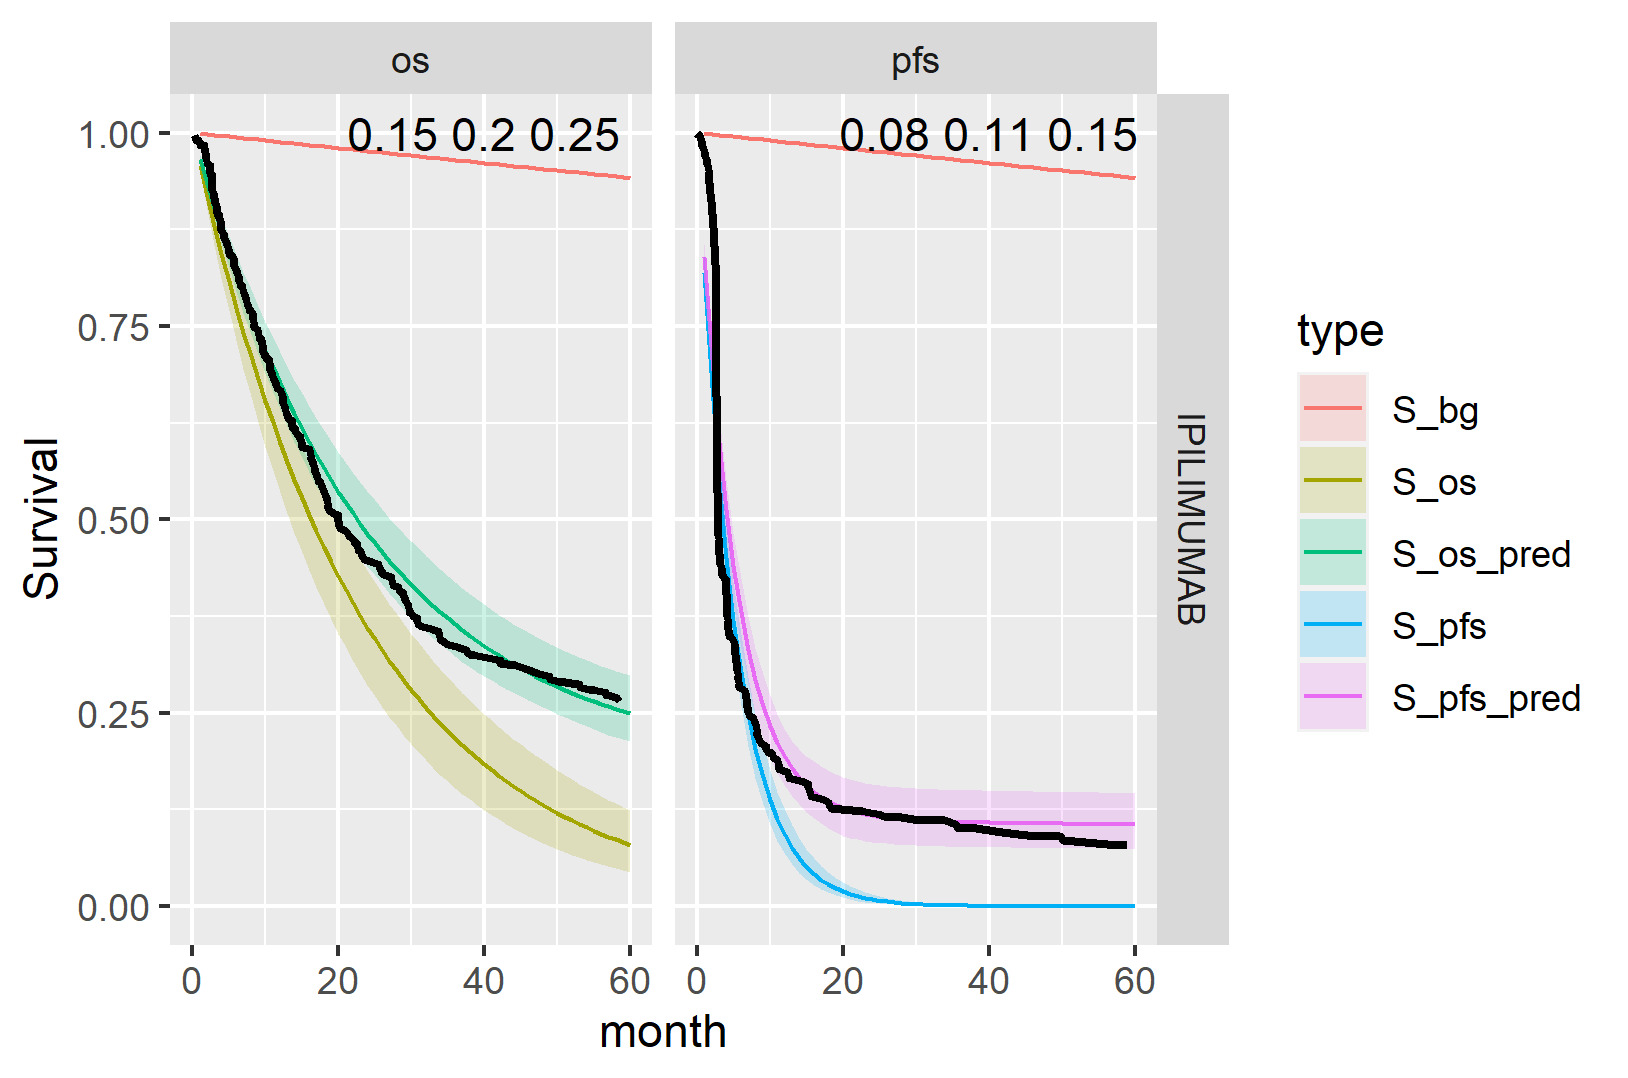
\includegraphics[width=0.4\linewidth]{../plots/S_plots_exp_exp_cf hier_bg_fixed_IPILIMUMAB} \end{center}

\begin{center}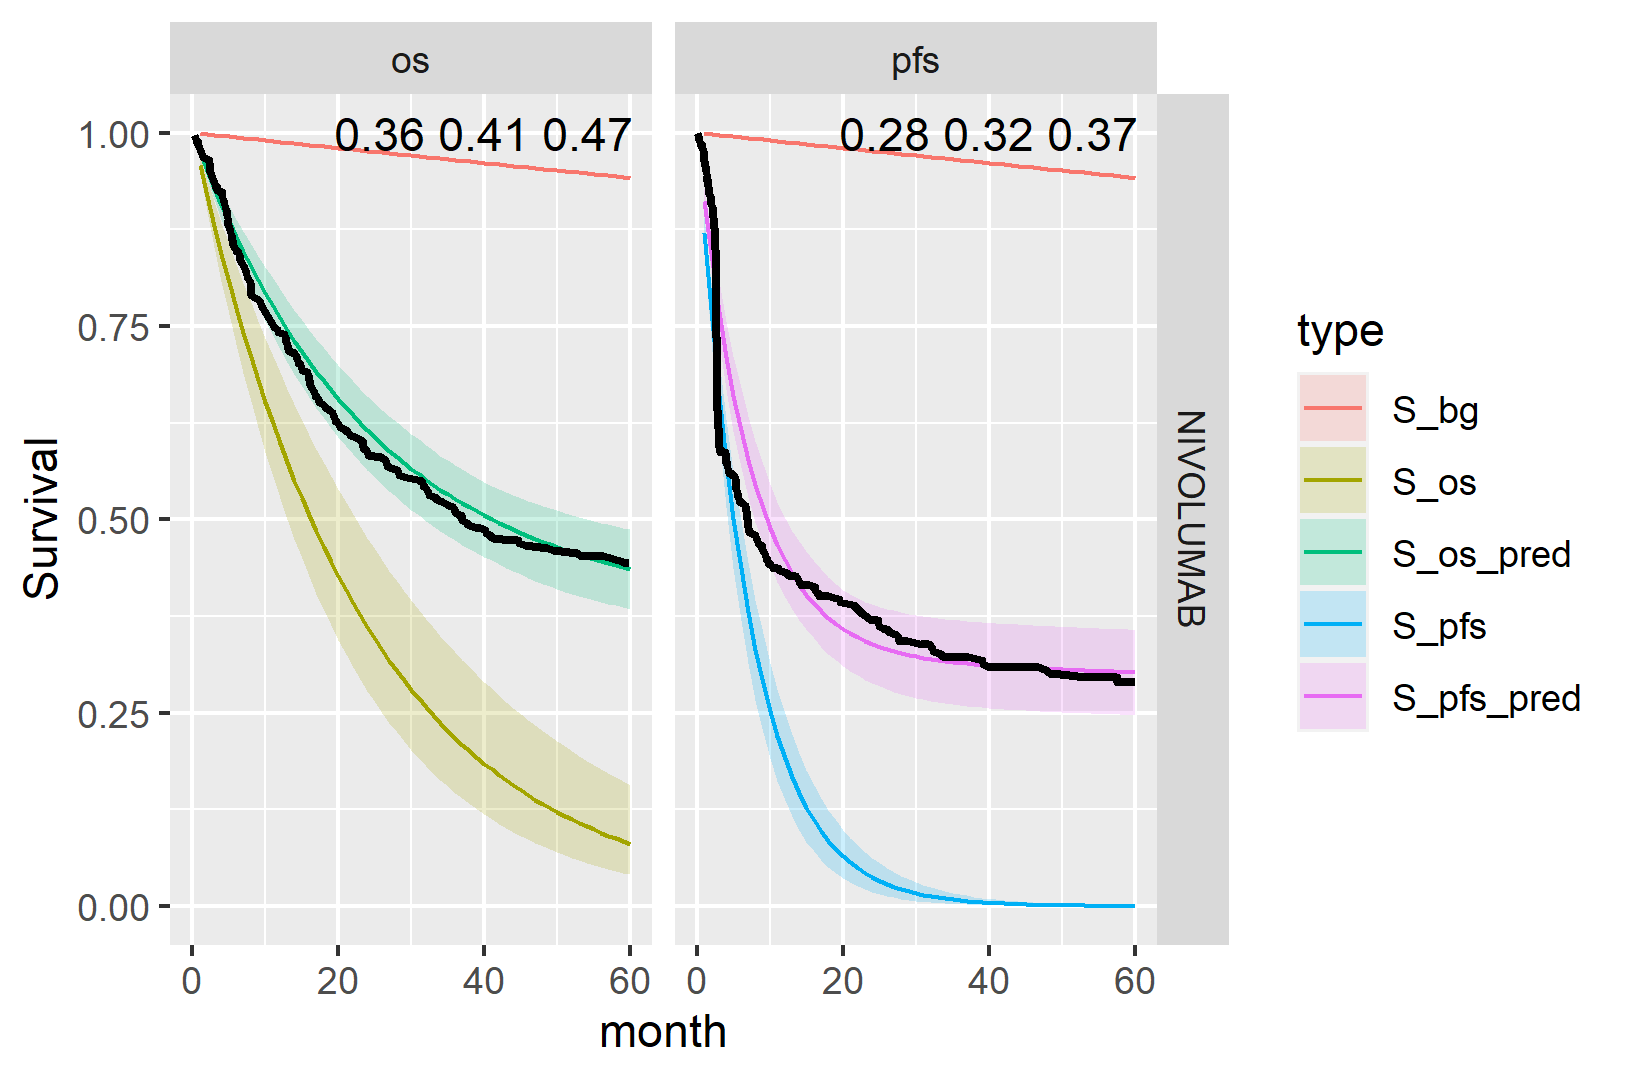
\includegraphics[width=0.4\linewidth]{../plots/S_plots_exp_exp_cf hier_bg_fixed_NIVOLUMAB} \end{center}

\begin{center}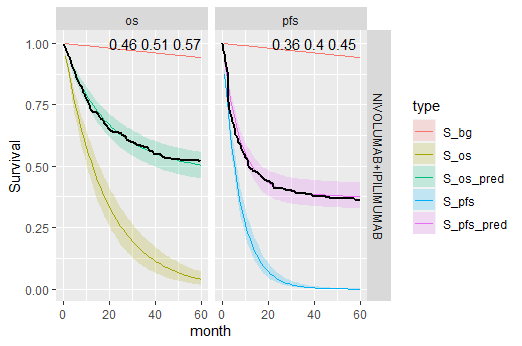
\includegraphics[width=0.4\linewidth]{../plots/S_plots_exp_exp_cf_hier_bg_fixed_NIVO+IPI} \end{center}

The table below summarises the cure fraction posterior distribution for
each scenario.

\begin{longtable}[]{@{}lrrrrrr@{}}
\toprule
\begin{minipage}[b]{0.01\columnwidth}\raggedright
\strut
\end{minipage} & \begin{minipage}[b]{0.10\columnwidth}\raggedleft
Event times\strut
\end{minipage} & \begin{minipage}[b]{0.12\columnwidth}\raggedleft
Cure fraction\strut
\end{minipage} & \begin{minipage}[b]{0.09\columnwidth}\raggedleft
Treatment\strut
\end{minipage} & \begin{minipage}[b]{0.16\columnwidth}\raggedleft
\(cf\) (CrI)\strut
\end{minipage} & \begin{minipage}[b]{0.16\columnwidth}\raggedleft
\(cf_{OS}\) (CrI)\strut
\end{minipage} & \begin{minipage}[b]{0.16\columnwidth}\raggedleft
\(cf_{PFS}\) (CrI)\strut
\end{minipage}\tabularnewline
\midrule
\endhead
\begin{minipage}[t]{0.01\columnwidth}\raggedright
1\strut
\end{minipage} & \begin{minipage}[t]{0.10\columnwidth}\raggedleft
Independent\strut
\end{minipage} & \begin{minipage}[t]{0.12\columnwidth}\raggedleft
Hierarchical\strut
\end{minipage} & \begin{minipage}[t]{0.09\columnwidth}\raggedleft
IPI\strut
\end{minipage} & \begin{minipage}[t]{0.16\columnwidth}\raggedleft
0.151 (0.068, 0.26)\strut
\end{minipage} & \begin{minipage}[t]{0.16\columnwidth}\raggedleft
0.196 (0.136, 0.255)\strut
\end{minipage} & \begin{minipage}[t]{0.16\columnwidth}\raggedleft
0.112 (0.079, 0.155)\strut
\end{minipage}\tabularnewline
\begin{minipage}[t]{0.01\columnwidth}\raggedright
2\strut
\end{minipage} & \begin{minipage}[t]{0.10\columnwidth}\raggedleft
Independent\strut
\end{minipage} & \begin{minipage}[t]{0.12\columnwidth}\raggedleft
Hierarchical\strut
\end{minipage} & \begin{minipage}[t]{0.09\columnwidth}\raggedleft
NIVO\strut
\end{minipage} & \begin{minipage}[t]{0.16\columnwidth}\raggedleft
0.378 (0.216, 0.557)\strut
\end{minipage} & \begin{minipage}[t]{0.16\columnwidth}\raggedleft
0.412 (0.35, 0.479)\strut
\end{minipage} & \begin{minipage}[t]{0.16\columnwidth}\raggedleft
0.321 (0.262, 0.379)\strut
\end{minipage}\tabularnewline
\begin{minipage}[t]{0.01\columnwidth}\raggedright
3\strut
\end{minipage} & \begin{minipage}[t]{0.10\columnwidth}\raggedleft
Independent\strut
\end{minipage} & \begin{minipage}[t]{0.12\columnwidth}\raggedleft
Hierarchical\strut
\end{minipage} & \begin{minipage}[t]{0.09\columnwidth}\raggedleft
NIVO+IPI\strut
\end{minipage} & \begin{minipage}[t]{0.16\columnwidth}\raggedleft
0.463 (0.322, 0.62)\strut
\end{minipage} & \begin{minipage}[t]{0.16\columnwidth}\raggedleft
0.519 (0.448, 0.585)\strut
\end{minipage} & \begin{minipage}[t]{0.16\columnwidth}\raggedleft
0.398 (0.336, 0.455)\strut
\end{minipage}\tabularnewline
\bottomrule
\end{longtable}

Leave-one-out cross validation statistics:

\begin{longtable}[]{@{}rrrr@{}}
\toprule
& stat & Estimate & SE\tabularnewline
\midrule
\endhead
IPI & elpd\_waic & -1838.826318 & 36.0674047\tabularnewline
NIVO & elpd\_waic & -1679.593315 & 45.6855459\tabularnewline
IPI+NIVO & elpd\_waic & -1543.235582 & 53.8029923\tabularnewline
IPI & p\_waic & 5.373491 & 0.4815243\tabularnewline
NIVO & p\_waic & 7.452234 & 0.6225800\tabularnewline
IPI+NIVO & p\_waic & 6.671215 & 0.5213592\tabularnewline
IPI & waic & 3677.652636 & 72.1348094\tabularnewline
NIVO & waic & 3359.186630 & 91.3710918\tabularnewline
IPI+NIVO & waic & 3086.471164 & 107.6059845\tabularnewline
\bottomrule
\end{longtable}

The variance partition coefficient (VPC) is defined as
\(\sigma_{global}^2/ (\sigma_{global}^2 + \sigma_{e}^2)\) where
\(e = PFS\) or \(OS\).

\begin{longtable}[]{@{}rrr@{}}
\toprule
& PFS & OS\tabularnewline
\midrule
\endhead
IPI & 0.8132749 & 0.7838815\tabularnewline
NIVO & 0.8760108 & 0.8765306\tabularnewline
IPI+NIVO & 0.8571695 & 0.8459290\tabularnewline
\bottomrule
\end{longtable}

\hypertarget{future-work}{%
\subsection{Future work}\label{future-work}}

\hypertarget{expand-available-distributions}{%
\paragraph{Expand available
distributions}\label{expand-available-distributions}}

Having shown the application of these methods to this problem we will
extend the tool kit to include other standard parametric distributions
are tested:

\begin{itemize}
\tightlist
\item
  Weibull
\item
  Gompertz
\item
  Log-normal
\item
  Log-logistic
\item
  Generalised gamma
\end{itemize}

\hypertarget{sensitivity-analysis}{%
\paragraph{Sensitivity analysis}\label{sensitivity-analysis}}

Of course, when the data offer only limited amount of information, the
assumptions in the prior distribution possibly exert much influence on
the results - and crucially on the decision model output. We will
conduct extensive sensitivity analysis and will justify assumptions in
all aspects of the modelling strategy by assessing the meaning of the
various distributional assumptions visually and formally.

\hypertarget{model-checking-and-testing}{%
\paragraph{Model checking and
testing}\label{model-checking-and-testing}}

We have already written a suite of simulation functions to create
synthetic cohorts with which to test the models such that we know the
true underlying data generating process.

\hypertarget{background-survival-1}{%
\paragraph{Background survival}\label{background-survival-1}}

An alternative non-parametric approach, as used in Demiris and Sharples
(2006), is to use a \emph{Gamma process} to define gamma distributions
at each time. A variance parameter determines the influence between
times.

Average values derived from the life tables are used in the Gamma
process. These are age-sex-country standardised. The below plot shows
the mean, median and a sample of hazard curves for the checkmate data
set. The underlying hazard curve for 0-100 year olds is shifted left
depending on the starting age of an individual in the cohort.

\begin{center}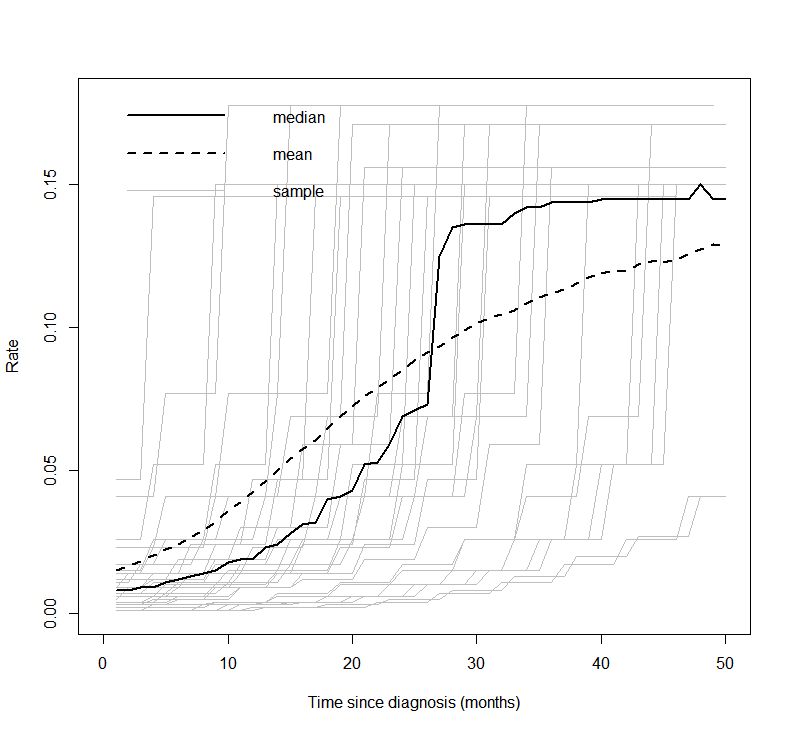
\includegraphics[width=0.6\linewidth]{../docs/background_average_rate_plot} \end{center}

\hypertarget{additional-model-structure}{%
\paragraph{Additional model
structure}\label{additional-model-structure}}

The two regression models can be extended to more complex structures,
for instance by including a mixture model in one or both (and eventually
by including some further correlation structure in the mixing
parameters).

For this analysis it was unnecessary but we may generalise the model so
that the cure fraction is dependent on covariates. Therefore, the
posterior with \(\beta^{cf}\) representing the coefficients of the cure
fraction regression is

\[
p(\boldsymbol{\beta^u},\boldsymbol{\beta^*}, \boldsymbol{\beta^{cf}} | \boldsymbol{\delta}, \boldsymbol{x}) \propto L(\boldsymbol{\beta^u},\boldsymbol{\beta^*}, \boldsymbol{\beta^{cf}} | \boldsymbol{\delta}, \boldsymbol{x}) g_1(\boldsymbol{\beta^{cf}})  g_2(\boldsymbol{\beta^u}) g_3(\boldsymbol{\beta^*})
\]

\hypertarget{references}{%
\subsection*{References}\label{references}}
\addcontentsline{toc}{subsection}{References}

\hypertarget{refs}{}
\begin{CSLReferences}{1}{0}
\leavevmode\hypertarget{ref-Amico2018}{}%
Amico, Maïlis, and Ingrid Van Keilegom. 2018. {``{Cure Models in
Survival Analysis}.''} \emph{Annual Review of Statistics and Its
Application} 5: 311--42.
\url{https://doi.org/10.1146/annurev-statistics-031017-100101}.

\leavevmode\hypertarget{ref-carpenter2017stan}{}%
Carpenter, Bob, Andrew Gelman, Matthew D Hoffman, Daniel Lee, Ben
Goodrich, Michael Betancourt, Marcus Brubaker, Jiqiang Guo, Peter Li,
and Allen Riddell. 2017. {``Stan: A Probabilistic Programming
Language.''} \emph{Journal of Statistical Software} 76 (1).

\leavevmode\hypertarget{ref-Demiris2006}{}%
Demiris, Nikolaos, and Linda D. Sharples. 2006. {``{Bayesian evidence
synthesis to extrapolate survival estimates in cost-effectiveness
studies}.''} \emph{Statistics in Medicine} 25 (11): 1960--75.
\url{https://doi.org/10.1002/sim.2366}.

\leavevmode\hypertarget{ref-wholifetables}{}%
WHO. 2020. {``{Life tables by country}.''}
\url{http://apps.who.int/gho/data/?theme=main\&vid=61160}.

\end{CSLReferences}

\end{document}
